% =====================================================================
%  State-of-the-project report, TUEG VLM prediction
%  Build:  tectonic report/project-report.tex
% =====================================================================
\documentclass[11pt,a4paper]{article}

% --- fonts -----------------------------------------------------------
\usepackage{libertinus}          % serif + sans + mono + math, one family
\usepackage{microtype}
\usepackage[htt]{hyphenat}       % never hyphenate inside \texttt (file paths)

% --- page ------------------------------------------------------------
\usepackage[margin=2.0cm,top=2.3cm,bottom=2.0cm]{geometry}
\usepackage{booktabs}
\usepackage{array}
\usepackage{longtable}
\usepackage{graphicx}
\usepackage{xcolor}
\usepackage{enumitem}
\usepackage{caption}
\usepackage{titlesec}
\usepackage{fancyhdr}
\usepackage[most]{tcolorbox}
\usepackage{tikz}
\usetikzlibrary{arrows.meta,positioning,calc}
\usepackage[colorlinks,linkcolor=accent,citecolor=accent,urlcolor=accent]{hyperref}

% --- palette ---------------------------------------------------------
\definecolor{ink}{HTML}{1A1D21}
\definecolor{accent}{HTML}{1F3A5F}
\definecolor{rule}{HTML}{D5DAE0}
\definecolor{panel}{HTML}{F5F7F9}
\definecolor{muted}{HTML}{5F6B78}
\definecolor{ok}{HTML}{2E6E4E}
\definecolor{warn}{HTML}{8A6100}
\definecolor{stop}{HTML}{8C3A2E}
\definecolor{idle}{HTML}{6B7280}

\color{ink}

% --- headings --------------------------------------------------------
\titleformat{\section}
  {\normalfont\sffamily\large\bfseries\color{accent}}
  {\thesection}{0.7em}{}[{\vspace{2pt}\color{rule}\titlerule[0.6pt]}]
\titleformat{\subsection}
  {\normalfont\sffamily\normalsize\bfseries\color{ink}}
  {\thesubsection}{0.6em}{}
\titlespacing*{\section}{0pt}{1.15em}{0.45em}
\titlespacing*{\subsection}{0pt}{0.75em}{0.25em}

\captionsetup{font=small,labelfont={sf,bf,color=accent},skip=5pt}
\setlist[itemize]{leftmargin=1.15em,itemsep=0.20em,topsep=0.25em}
\setlist[enumerate]{leftmargin=1.45em,itemsep=0.20em,topsep=0.25em}

\emergencystretch=2em
\tolerance=1200
\setlength{\parskip}{0.28em}
\setlength{\parindent}{0pt}
\renewcommand{\arraystretch}{1.15}

% --- running head ----------------------------------------------------
\pagestyle{fancy}\fancyhf{}
\renewcommand{\headrulewidth}{0.4pt}
\renewcommand{\headrule}{\color{rule}\hrule height 0.4pt}
\fancyhead[L]{\footnotesize\sffamily\color{muted}TUEG\,/\,VLM benchmark}
\fancyhead[R]{\footnotesize\sffamily\color{muted}17 August 2026}
\fancyfoot[C]{\footnotesize\sffamily\color{muted}\thepage}

% --- components ------------------------------------------------------
\newcommand{\file}[1]{{\small\texttt{#1}}}

% status chip
\newcommand{\chip}[2]{%
  \tikz[baseline=(c.base)]{\node[inner xsep=4.5pt,inner ysep=1.8pt,rounded corners=2pt,
    fill=#1!11,text=#1!78!black,font=\scriptsize\sffamily\bfseries] (c) {#2};}}

% headline-number tile
\newcommand{\tile}[2]{%
  \begin{minipage}[t]{0.24\linewidth}\centering
    {\large\sffamily\bfseries\color{accent}#1}\\[0.1em]
    {\scriptsize\sffamily\color{muted}#2}
  \end{minipage}}

\newtcolorbox{summarybox}{
  enhanced, breakable, boxrule=0pt, frame hidden,
  colback=panel, arc=2pt, left=10pt, right=10pt, top=8pt, bottom=8pt,
  borderline west={2.2pt}{0pt}{accent}}

\newtcolorbox{notebox}[1]{
  enhanced, breakable, boxrule=0.5pt, colframe=rule,
  colback=white, arc=2pt, left=8pt, right=8pt, top=6pt, bottom=6pt,
  fonttitle=\footnotesize\sffamily\bfseries\color{accent},
  coltitle=accent, colbacktitle=white, title=#1,
  attach boxed title to top left={xshift=8pt,yshift=-\tcboxedtitleheight/2},
  boxed title style={boxrule=0pt,colback=white,left=3pt,right=3pt}}

\begin{document}
\thispagestyle{fancy}

\begingroup
\setlength{\parskip}{0pt}
{\LARGE\bfseries\color{accent}Benchmarking Off-the-Shelf Vision--Language Models\\[0.18em]
on EEG Waveform Images\par}
\vspace{0.55em}
{\large\sffamily\color{muted}Technical and architectural state of the project\par}
\vspace{0.7em}
{\color{rule}\hrule height 0.8pt}
\vspace{0.55em}
{\small\sffamily\color{muted}Luka\quad\textbullet\quad\texttt{lukaj2501@gmail.com}\quad\textbullet\quad 17 August 2026\par}
\endgroup
\vspace{1.1em}

\begin{summarybox}
EEG recordings from six sub-corpora of the Temple University EEG Corpus are
rendered as multi-channel waveform plots and shown to 35 off-the-shelf
vision--language models (VLMs), which are asked to classify them with no
EEG-specific training. Everything runs through Ollama as Slurm array jobs on
Narval. A second track fine-tunes a small model on written rationales produced by
a larger one.

\smallskip
The corpus and the evaluation harness are complete. The full sweep has not been
run yet, so this report describes the system and the reasoning behind it.
Section~\ref{sec:status} lists what is finished and what is still missing.
\end{summarybox}

\vspace{0.5em}
\noindent
\tile{76{,}334}{rendered windows}\hfill
\tile{35 $\times$ 6}{models $\times$ corpora}\hfill
\tile{210}{array tasks}\hfill
\tile{14{,}850}{windows scored}
\vspace{0.4em}

% =====================================================================
\section{What the project is testing}
% =====================================================================

The question is how well a general-purpose vision model can read an EEG when it
is presented the way a clinician sees it, as a stacked plot of every channel
against time. None of these models were trained on EEG, so the measurement is how
far general multimodal capability transfers to an image type well outside the
training distribution.

The framing needs to stay precise. Rendering a 40-channel signal as a picture
discards fine morphology that a model reading the raw 1-D signal keeps, so a
specialised EEG classifier should be expected to win. The useful comparison is
not against that classifier but against what a model scores by ignoring the image
entirely, which is why a constant-predictor baseline accompanies every result
(Section~\ref{sec:scoring}).

\begin{figure}[h]
\centering
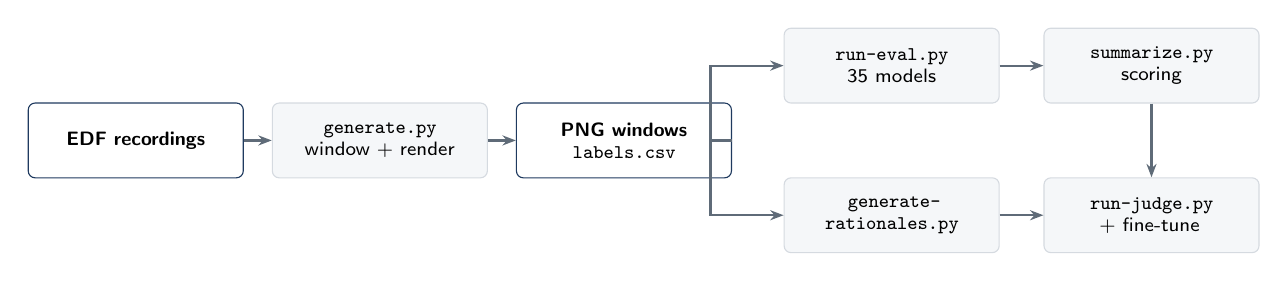
\begin{tikzpicture}[
  x=1cm,y=1cm,
  b/.style={draw=rule,fill=panel,rounded corners=2.5pt,inner sep=4pt,align=center,
            font=\scriptsize\sffamily,text width=2.45cm,minimum height=0.95cm},
  d/.style={b,draw=accent,fill=white,font=\scriptsize\sffamily\bfseries},
  a/.style={-{Stealth[length=1.7mm]},draw=muted,thick},
  n/.style={font=\tiny\sffamily\bfseries,color=muted}]
\node[d] (edf)  at (0,0)     {EDF recordings};
\node[b] (gen)  at (3.1,0)   {\texttt{generate.py}\\ window + render};
\node[d] (png)  at (6.2,0)   {PNG windows\\ \texttt{labels.csv}};
\node[b] (ev)   at (9.6,0.95) {\texttt{run-eval.py}\\ 35 models};
\node[b] (sum)  at (12.9,0.95){\texttt{summarize.py}\\ scoring};
\node[b] (rat)  at (9.6,-0.95){\texttt{generate-}\\\texttt{rationales.py}};
\node[b] (jud)  at (12.9,-0.95){\texttt{run-judge.py}\\ + fine-tune};
\draw[a] (edf)--(gen); \draw[a] (gen)--(png);
\draw[a] (png.east)--(7.3,0)|-(ev.west);
\draw[a] (png.east)--(7.3,0)|-(rat.west);
\draw[a] (ev)--(sum); \draw[a] (rat)--(jud);
\draw[a] (sum.south)--(12.9,0)--(jud.north);
\end{tikzpicture}
\caption{Stage layout. White boxes are durable artifacts on disk, grey boxes are
stages. Every long-running stage resumes from partial progress, because these run
as array jobs on a shared cluster where a requeue can cost days.}
\end{figure}

% =====================================================================
\section{Cluster environment}
% =====================================================================

All GPU work runs on Narval (Digital Research Alliance of Canada, account
\texttt{def-milad777}), whose GPU nodes carry A100-40\,GB cards and support MIG.
MIG (Multi-Instance GPU) partitions one physical card into hardware-isolated
slices, each with its own memory and compute units, so several jobs share a card
without contending for it. The project uses MIG heavily: a small model takes a
20\,GB slice rather than occupying a whole 40\,GB card.

That is not a stylistic preference. Early in development the project drew a
resource-waste warning from the cluster operators for under-utilised full-GPU
jobs, and most of the resource engineering described below is the response to it.

Work is submitted as Slurm \emph{array jobs}: one submission expands into $N$
indexed tasks that the scheduler places independently, so 210 model-and-dataset
pairs queue as eleven submissions rather than 210.

\subsection{Ollama}

Inference is served by Ollama running inside an Apptainer container. Apptainer is
the HPC container runtime (formerly Singularity) that runs unprivileged, so a
user can bring their own userspace onto a compute node. It is required here
because the native \texttt{ollama} binary is not on Narval's compute-node
\texttt{PATH}; assuming it was there once left a rationale job spinning until its
walltime expired. Two paths on scratch are the only manual setup step in the
whole project: \file{\$SCRATCH/ollama/ollama.sif} (the container image, built
once) and \file{\$SCRATCH/ollama/models} (the model store, shared by every job).

Every array task starts its own Ollama server. The port is derived from the job
and task IDs as \texttt{20000 + (job + task) mod 40000}, so two tasks landing on
one node cannot collide, and a shell trap kills the server on exit. The task
waits up to 120\,s for the server to answer and records the Ollama version
alongside the run, since vision-model regressions land there often enough to
matter (0.13.3 broke image input outright, \texttt{ollama/ollama\#13549}).

Three settings are exported into the container, each read from the same place the
Python client reads it so that server and client cannot disagree:

\begin{itemize}
\item \textbf{Requests in flight} (8 on a full A100, 4 on a MIG slice). Ollama
      batches concurrent requests, so this is what keeps the GPU busy instead of
      idling between images.
\item \textbf{Context length} 8192. An image plus prompt is about 4{,}000 tokens,
      and the 4096 default truncated output mid-rationale.
\item \textbf{Flash attention.} Flash attention is an attention kernel that
      computes attention in tiles kept in fast on-chip memory and never
      materialises the full $N \times N$ attention matrix, so memory use falls
      from quadratic to linear in sequence length and decoding is faster. Here it
      is enabled less for the speed than as a bug workaround: on the non-flash
      path Ollama never emits an end-of-sequence token on Qwen2.5-VL, and the
      reply runs to the token limit.
\end{itemize}

\begin{notebox}{Compute nodes have no outbound network}
Neither \texttt{registry.ollama.ai} nor \texttt{huggingface.co} is reachable from
a compute node, so every model must be staged into \file{\$SCRATCH/ollama/models}
from a login node \emph{before} submission. This is a staging step, not a
limitation to engineer around, but it has teeth: a \texttt{pull} fallback inside a
compute-node job can only hang and then time out, reporting a network error
rather than ``model not staged''. That cost a whole judge array on 16 August. The
sbatch wrappers now fail fast and name the missing model, and
\file{run-judge.py check} verifies staging before anything is queued.
\end{notebox}

\subsection{Hugging Face weights}

Ollama serves quantised GGUF weights. GGUF is a single-file weight format packed
for llama.cpp-style inference: fine for serving, but the tensors cannot be fed to
a PyTorch LoRA fine-tune. LoRA (low-rank adaptation) freezes the base weights and
trains a small pair of low-rank matrices alongside them, which needs the original
full-precision checkpoint. \file{hf-install.py} therefore downloads complete
Hugging Face snapshots (weights, processor, chat template) for the fine-tune
track, keeping an explicit map from Ollama tag to HF checkpoint and writing a
manifest.

It runs from a \textbf{login node}, because it needs outbound internet and
compute nodes have none. Downloading all of it in one pass did not work: roughly
forty repositories, several of them tens of gigabytes, with parallel connections,
decompression and hashing throughout, exceeded what a shared login node permits
one user, and the run died with an error partway through. The fix was not to make
the script cheaper but to run it repeatedly over a handful of repositories at a
time; \file{hf-install.py} checks each repository against the current remote
revision and skips any already complete on disk, so a re-run costs only the
remainder. The downloads were spread across roughly a week that way. Gated
repositories need their licence accepted on Hugging Face first, and fail loudly
until it is.

A Slurm wrapper for the script is in git history, but a compute node cannot reach
Hugging Face, so the login-node path above is the working one. Both files are
currently deleted from the working tree and need restoring before the fine-tune
track can proceed (Section~\ref{sec:status}).

% =====================================================================
\section{Dataset generation}
% =====================================================================

\subsection{Download and layout}

Source corpora are pulled from Temple's ISIP server with
\file{eval/scripts/download.sh}, a thin wrapper over \texttt{rsync -auvxL} so that
an interrupted transfer resumes instead of restarting, which matters when TUSZ
alone is roughly 85\,GB of EDF. (EDF, European Data Format, is the standard
clinical container for a multi-channel recording plus its per-channel metadata.)
Each corpus unpacks into its own versioned directory inside its dataset folder,
the layout the generators expect. \file{<CORPUS>} below is one of \texttt{TUAB},
\texttt{TUAR}, \texttt{TUEP}, \texttt{TUEV}, \texttt{TUSL}, \texttt{TUSZ}:

\begin{center}\small
\begin{tabular}{@{}ll@{}}
\toprule
\textbf{\sffamily Path} & \textbf{\sffamily Contents} \\
\midrule
\file{datasets/<CORPUS>/v*.*.*/} & raw EDF, never committed \\
\file{datasets/<CORPUS>/generate.py} & dataset-specific label logic and split \\
\file{datasets/<CORPUS>/labels.csv} & the manifest, committed to git \\
\file{datasets/<CORPUS>/\{train,test\}/} & rendered PNG windows, shipped by zip \\
\file{datasets/\_render.py} & shared windowing and rendering engine \\
\file{datasets/generate-all.sh} & runs all six generators in parallel \\
\bottomrule
\end{tabular}
\end{center}

Images and labels reach the cluster by different routes, which is worth knowing
before changing either. \file{labels.csv} travels via git, the images as a
37.7\,GB zip bundle. A label change is therefore a \texttt{git pull}; an image
change means re-zipping and re-transferring everything.

\subsection{Splitting and windowing}

\file{generate-all.sh} runs the six \file{generate.py} scripts in parallel, each
writing to its own directory. Each generator supplies four dataset-specific
pieces (how to read the patient ID from a filename, how to name scans, how to
split, and how to label a time range) and delegates the rest to the shared
engine.

The split is 70/30 and grouped by \emph{patient}. Patients are sorted, shuffled
with a fixed seed, and assigned whole to test until about 30\% of scans is
reached, so every recording and window from one person lands on the same side.
This is what stops a model being rewarded for recognising an individual's EEG
instead of the finding, and it is deterministic given the seed.

Recordings run from 4 to 50 minutes, which creates the central sampling problem.
Rendering an entire recording into one image yields roughly one pixel per second
and destroys the morphology the task depends on, so recordings are cut into
non-overlapping 20-second windows. Rendering every window would then produce
hundreds of thousands of images, so the two splits use different policies:

\begin{itemize}
\item \textbf{Train} takes a small mixed sample per recording (4 windows by
      default, seeded per recording): windows containing an annotated event are
      preferred, and the remainder is filled with background. The model sees both
      the finding and normal activity, cheaply.
\item \textbf{Test} takes evenly-spaced background windows (capped at 10) plus
      \emph{every} window containing an event. The test set therefore resembles
      the recording as a whole while still guaranteeing that rare findings are
      present.
\end{itemize}

An earlier version rendered only the first 20 seconds of each recording and
missed events almost entirely, which is what motivated this design.

\subsection{Rendering}

Rendering is centralised in \file{datasets/\_render.py} so that images are
comparable across all six datasets. Each recording is read once with MNE (the
standard Python library for EEG and MEG) using
\texttt{read\_raw\_edf(preload=True)}. Eager preloading is required because TUEG
files mix sampling rates across channels, and lazily loaded mixed-rate data
produces edge artifacts at window boundaries. A 0.5--70\,Hz bandpass and a
60\,Hz notch (a narrow cut at the North American mains frequency) are applied once
per recording, removing drift and line hum so that recordings from different
machines are comparable. Marker channels such as \texttt{IBI} and
\texttt{PHOTIC} are skipped, since filtering a derived channel produces ringing.

Every channel gets its own subplot row, 30 to 41 rows per image, so traces never
overlap. Images are $16\times16$ inches at 96\,dpi, giving exactly
$1536\times1536$\,px. A VLM cuts an image into patches and charges each patch
against its context, so resolution is a direct cost: this one is about 3{,}050
vision tokens. Legibility turned out to depend on font size and not on pixel
count. 1536 and 2048\,px produced identical read-back, while raising channel
labels from 5\,pt to 8\,pt bold fixed it, and models now read back roughly 26 of
30 channel labels correctly.

Two further decisions shape what the models can see.

\textbf{Amplitude is scaled per channel}, to the 99th percentile of $|y|$ times
1.15. Getting there took three attempts: scaling to the median clipped badly
(EEG has a crest factor around 12), and $8\times$ median overcorrected and buried
the trace at roughly 12\% of the row height, which reads as a flat line. Global
scaling across channels was prototyped and rejected outright, because channels
differ in amplitude by up to $25\times$ and the loud ones become unreadable solid
blocks. The trade is that cross-channel amplitude comparison is lost, so
asymmetry and attenuation cues are unavailable and a scale bar would be
meaningless.

\textbf{Nothing in the image identifies the answer.} The EDF filename is never
drawn on the plot. An early version used it as the title, and because TUEG
filenames encode the class for several corpora (\texttt{pled\_...},
\texttt{normal/...}), models could read the answer straight off the image. Output
files are named \texttt{<patient>\_<scan>\_<window>.png}, carrying no label and no
dataset.

\subsection{\file{labels.csv} and the \texttt{assessed} flag}

Each dataset directory holds one manifest with a row per rendered window: the
image path, the split, one boolean column per class, and an \texttt{assessed}
flag. It is streamed as rendering proceeds, so a completed run leaves a complete
manifest and a crashed one leaves an obviously partial file.

The \texttt{assessed} flag exists because of a label-quality problem found after
the images already existed. The label function returned an empty set both when
annotators had marked a window quiet and when they had never examined it, and
generation wrote both as an all-false row. Scoring therefore graded
never-inspected windows as though every class were absent, so they could only
ever generate false positives and could never contribute to recall. This affected
roughly 70\% of TUSZ, 79\% of TUEV and 75\% of TUSL test windows.

Which meaning applies proved measurable per corpus, and the two cases get
opposite treatment. TUSZ never mixes them in one annotation file (of 8{,}140
files, 7{,}043 are background-only and 1{,}097 seizure-only, and none holds
both), and its seizure annotations are provably complete: the local copy
reproduces the official \file{AAREADME.txt} event and duration statistics exactly.
So absence of annotation genuinely is background there, and those windows were
relabelled rather than dropped. TUEV, TUSL and TUAR annotate background
explicitly, so an unannotated window means nobody looked, and those are excluded
from scoring (\texttt{assessed=false} on 2{,}378 TUEV, 538 TUAR and 472 TUSL
windows; zero elsewhere).

TUAR had a second, separate problem: its generator discarded the 3{,}122
background rows present in the source annotations, leaving a class that the
prompt offered but that could never be correct, and a test set with no true
negatives at all. They were recovered under a gate that refuses to write unless
every pre-existing label first reproduces exactly from source.

Both corrections were pure \file{labels.csv} transforms with no image
re-rendered, since a window's time span follows from its filename index and its
recording from the generator's deterministic naming.

\begin{table}[h]
\centering\small
\caption{The corpus as it stands, re-derived from \file{labels.csv} and
\file{eval/scripts/sample.py} on 17 August 2026. ``Assessed'' excludes windows no
annotator examined; ``sampled'' is the subset actually scored
(Section~\ref{sec:sampling}).}
\begin{tabular}{@{}lrrrrrrl@{}}
\toprule
\textbf{\sffamily Corpus} & \textbf{\sffamily Train} & \textbf{\sffamily Test} &
\textbf{\sffamily Assessed} & \textbf{\sffamily Sampled} & \textbf{\sffamily Rec.} &
\textbf{\sffamily Pat.} & \textbf{\sffamily Classes} \\
\midrule
TUAB & 2{,}800 & 3{,}000 & 3{,}000 & 1{,}200 & 300 & 222 & normal / abnormal \\
TUAR & 863 & 3{,}915 & 3{,}664 & 3{,}655 & 94 & 67 & 6 artifacts + bckg \\
TUEP & 6{,}868 & 8{,}610 & 8{,}610 & 1{,}084 & 285 & 113 & epilepsy / none \\
TUEV & 1{,}441 & 1{,}729 & 354 & 354 & 151 & 115 & 6 event types \\
TUSL & 312 & 400 & 99 & 97 & 34 & 8 & bckg / seiz / slow \\
TUSZ & 21{,}207 & 25{,}189 & 25{,}189 & 8{,}460 & 2{,}443 & 200 & bckg + 8 seizure types \\
\midrule
\textbf{Total} & \textbf{33{,}491} & \textbf{42{,}843} & \textbf{41{,}316} & \textbf{14{,}850} & & & \\
\bottomrule
\end{tabular}
\end{table}

\begin{figure}[h]
\centering
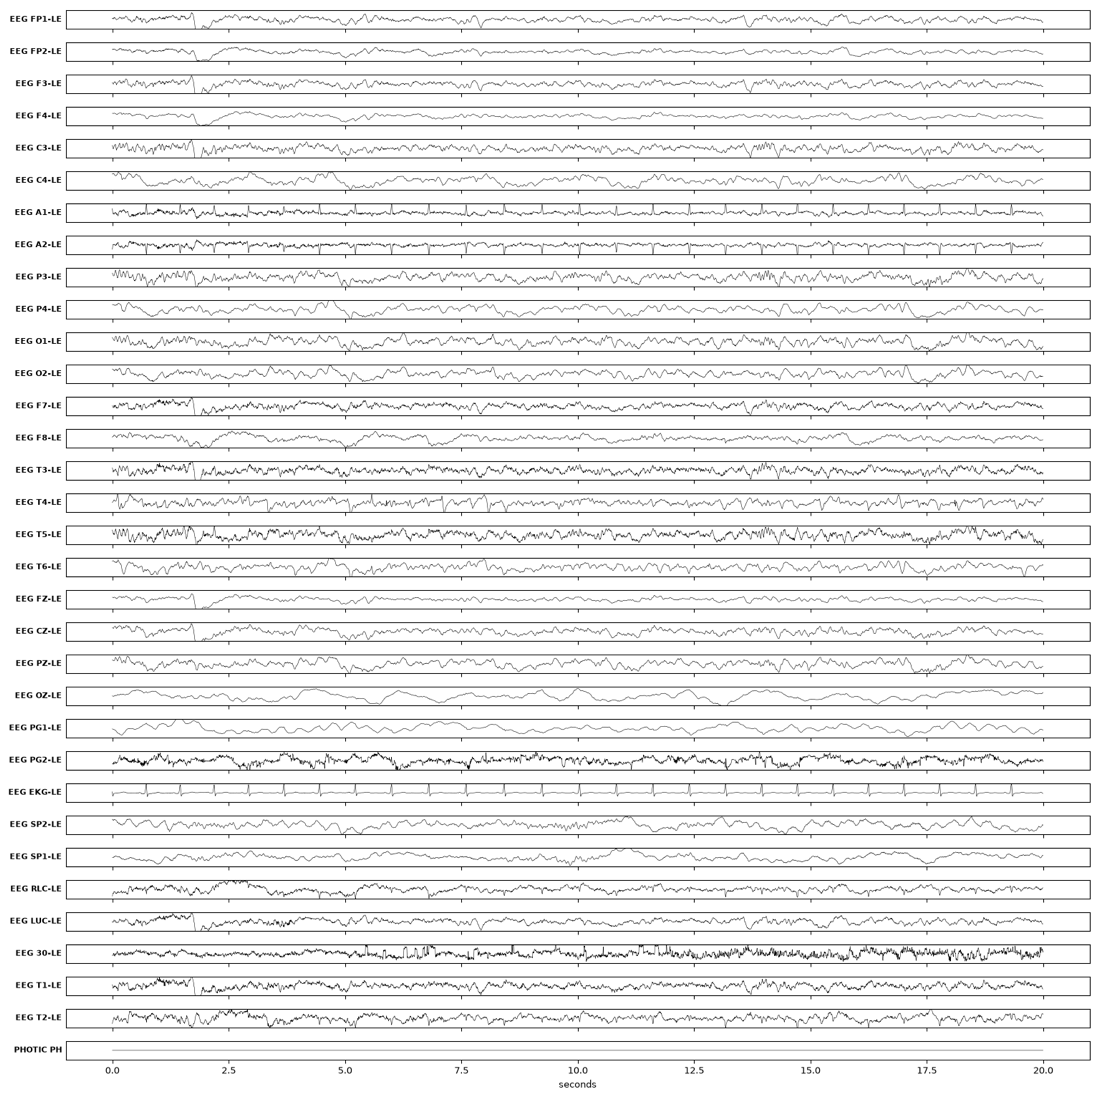
\includegraphics[width=0.40\linewidth]{figures/example-tusz-fnsz.png}
\caption{A representative model input: a 20-second window at
$1536\times1536$\,px with 31 channels on separate rows. Ground truth is
\texttt{fnsz}, a focal non-specific seizure. Nothing in the image or its filename
identifies the dataset, the class, or the source recording.}
\end{figure}

% =====================================================================
\section{Ground-truth rationale generation}
% =====================================================================

This stage shows a model the image \emph{together with the correct label} and
asks it to justify that label from visible evidence: which channel, where along
the time axis, and what the waveform looks like. The prompt forbids describing
the image format, defining terminology, or adding findings the label does not
contain.

The teacher is \texttt{gemma3:12b} at temperature 0, meaning greedy decoding:
the highest-probability token is taken at every step, so the same image always
produces the same rationale. It was originally a Qwen2.5-VL model, which had to
be replaced. In Ollama, Qwen2.5-VL falls into infinite single-token repetition on
these plots, and the bug affects the 7b, 32b and 72b variants alike
(\texttt{ollama/ollama\#10767}), so a larger Qwen is not the fix. Ollama also
exposes no repetition-loop detection (\texttt{\#16179}) and neither the DRY nor
the XTC sampler (\texttt{\#7504}), so no sampler setting prevents it either.
Changing model family was the only available lever.

One generator serves two consumers, selected by \texttt{--split}:
\file{rationales.csv} for the fine-tuning targets, and
\file{rationales-test.csv} for the reference rationales the judge compares
against. The separation is load-bearing, since the test file is derived from
held-out patients and training on it would void the patient split the whole
benchmark depends on.

The engineering here is mostly about not corrupting the output. A degenerate
reply, one too short or with too few distinct characters, is the signature of a
wedged runner, and because decoding is greedy it repeats identically on every
retry, so it passes every check except that one. Such a reply leaves the row blank
so a later run retries it, and 20 consecutive degenerate replies abort the job
rather than spending the rest of the allocation writing garbage into a
fine-tuning set. Each run also rebuilds its target list from the current
\file{labels.csv} while carrying over rationales already written, which fixed a
crash where a changed manifest desynchronised the lookup mid-job.

% =====================================================================
\section{Evaluation}
% =====================================================================

\subsection{Configuration}

\file{eval/config.yml} is the single source of configuration, with four keys:
\texttt{judge}, \texttt{settings}, \texttt{datasets} (the per-dataset prompts)
and \texttt{models} (the roster with per-model resources). One invariant matters,
because breaking it silently destroyed configuration once: every key the retry
generator loads, it must also write back.

Each dataset's prompt states that the image is a multi-channel EEG waveform plot
with one channel per row, names the exact label vocabulary, requires the model to
select every category present, and demands grounded per-item evidence. An earlier
generation of prompts described the images as spectrograms, which is wrong and
caused models to spend tokens noting the mismatch.

Predictions are never parsed from prose. \file{structure.py} builds a Pydantic
model per dataset, one boolean per class plus a rationale string, and that schema
is handed to the server as a JSON schema the decoder is constrained to satisfy.
So a reply is either valid structured output or an explicit failure, never a
paragraph to regex. It also bounds what the constant-predictor baseline is allowed
to propose.

\subsection{Test-set sampling}
\label{sec:sampling}

Compute scales with the number of windows, but statistical precision scales with
the scoring unit, which is the recording (the patient for TUEP). Densely tiling
background windows therefore consumes most of the compute while buying almost no
precision.

\file{sample.py} caps abundant label signatures at 3 windows per recording,
background-only windows at 2, binary-dataset windows at 4 per recording and
recordings at 4 per patient, while keeping every window carrying an
under-supported class in full. Selection is by even spacing with no RNG, so every
model is evaluated on an identical set that is reproducible from
\file{labels.csv} alone, with no sample file to go stale. After sampling, every
dataset's scoring-unit class support is identical to the full assessed set, so
the reduction from 41{,}316 to 14{,}850 windows costs nothing that gets reported.

\subsection{Dispatch and execution}

\file{run-eval.py} buckets the 210 \texttt{(model, dataset)} tasks by their
resource requirements into 11 groups, creates a run directory containing logs,
results, a status file and a frozen copy of the config, submits one Slurm array
per group, and records job and task IDs for later reconciliation. The roster
allocates 21 models to a 20\,GB MIG slice, 13 to a full A100, and one
mixture-of-experts model to four cards. (A mixture-of-experts model activates only
a fraction of its parameters per token but must still hold all of them resident,
so it is cheap to run and expensive to place.)

Three sizing rules decide whether a job runs at all, and all three are computed
rather than guessed:

\begin{itemize}
\item \textbf{VRAM}: $\text{weights} \times 1.15 + \text{KV cache} \times
      \text{requests in flight}$. Below that, Ollama silently offloads layers to
      CPU and runs orders of magnitude slower rather than failing.
\item \textbf{RAM}: $1.6 \times \text{weights} + 8$\,GB, and never above the
      \textasciitilde498\,GB a whole Narval GPU node has. Retuning these requests
      took the roster total from 2{,}488\,GB to 1{,}008\,GB, the single largest
      lever on queue wait.
\item \textbf{Walltime}: $2.5\times$ an estimated TUSZ task, TUSZ being the
      largest corpus and therefore the bound for all six. These are estimates, not
      measurements.
\end{itemize}

Ten further models sit commented out in the roster with their reason recorded:
three suspected Ollama tag aliases, five of the six \texttt{-thinking} variants
(the reasoning ablation is run once, at 8b, against the matching instruct model),
and two that do not fit the hardware. The clearest of those is
\texttt{qwen3-vl:235b-a22b}, whose Q4 weights are about 142\,GB against the
160\,GB of VRAM on four A100-40\,GB cards, leaving nothing for activations, the
vision tower or the KV cache; its earlier 512\,GB RAM request also exceeded the
node total, so that job could never have been scheduled at all. It is excluded
rather than deleted, and needs 80\,GB-class cards.

Each task decodes its model and dataset from the array index, starts Ollama,
restricts \file{labels.csv} to test patients, applies the sampling policy, and
runs the images through a thread pool sized to the model's in-flight setting.
Three behaviours are chosen on purpose. A per-image failure is logged and the run
continues, so one bad image cannot lose a task's work. Retries back off only for
transport errors, since a schema-validation failure is deterministic and pausing
before repeating it just burns walltime. And completed image paths are read from
both the current run and any previous run being resumed, so a Slurm requeue picks
up where it stopped.

\subsection{Retry, merge and monitoring}

Long jobs on a shared cluster fail partially, so three tools exist to make that
cheap to handle.

\file{status.py} reconciles the run's status file against live \texttt{squeue}
and \texttt{sacct} state and writes back outcomes for tasks that died without
recording their own failure, such as one killed by the walltime. It had a bug
worth recording: it asked \texttt{sacct} for \texttt{JobIDRaw}, which numbers
array \emph{elements} individually (\texttt{556372}) instead of
\texttt{<array>\_<task>} (\texttt{555281\_0}), so a guard on the underscore
skipped every finished element and the write-back never fired. Eleven tasks sat
at \texttt{running} against an empty queue before it was found.

\file{create-retry-config.py} rebuilds the config to re-run only the pairs that
failed and points \texttt{resume-from} at the run being retried. Finally,
\file{merge-runs.py} unions the base run and the retry into one scoreable
directory, and this step is not optional: \texttt{resume-from} only tells the
retry which images to skip and never copies base rows forward, so neither
directory is complete alone and scoring either one under-reports.

\subsection{Scoring}
\label{sec:scoring}

\file{summarize.py} is the single scoring stage. Two things motivate its design.
Accuracy on a background-dominated, window-tiled test set flatters a model that
always answers background. And TUAB and TUEP are labelled at the recording level,
so grading one normal-looking window against its recording's label is not a fair
unit.

The headline metric is therefore recording-level macro-F1: per-class F1 averaged
with every class weighted equally, so a rare seizure type counts as much as
background. A recording's windows are aggregated into one prediction, by majority
vote for the binary datasets and by any-positive detection for the multi-label
ones, and a class needs at least 20 positive recordings to enter the average.
Three guards accompany it:

\begin{itemize}
\item A 95\% bootstrap CI that resamples whole recordings rather than windows.
      Windows within a recording share a patient, montage and session, so
      resampling them individually would treat correlated observations as
      independent and understate the interval.
\item A constant-predictor baseline: the best macro-F1 an image-blind constant
      answer could achieve on the same data, restricted to answers the schema can
      emit. That restriction is not cosmetic, since TUAB and TUEP resolve to a
      single boolean, and allowing ``predict everything'' would put TUAB's floor
      at 0.666 instead of 0.346 and screen out every model.
\item A degeneracy flag for any model giving the same answer on 95\% or more of
      windows, and a descriptive-only marker for datasets with fewer than 20
      patients (TUSL has 8).
\end{itemize}

Scoring used to be two scripts, and the split was a trap worth naming. The
rigorous metrics were computed by one script that only printed them, while the
durable artifacts (\file{summary.csv}, \file{rank.csv}, \file{rank.png}) were
written by the other from window-level accuracy. The misleading view was the one
that persisted to disk and travelled into slides, and \file{rank.csv} ranked a
model that only ever answered ``background'' near the top. They are now one
script, verified equivalent before the old one was deleted, and the ranking sorts
on recording-level macro-F1.

Outputs are \file{summary.csv} (one row per model and dataset, carrying the
metrics together with \texttt{baseline\_macro\_f1}, \texttt{clears\_baseline},
\texttt{degenerate}, \texttt{few\_patients} and the task status, so a number
cannot be read without its caveat), \file{classes.csv}, \file{rank.csv} and one
ranking chart per dataset. The charts are per dataset rather than averaged
because a model carried by one easy dataset is indistinguishable, in a mean, from
one that transfers evenly. They plot recording-level balanced accuracy, whose
floor is a flat 0.50 for any image-blind constant answer and so needs no
accompanying explanation to be read correctly; macro-F1, which unlike balanced
accuracy charges a model for its false positives, remains the reported metric and
is what \file{rank.csv} ranks on. The sweep runs in two stages: all 35 models are screened on a
stratified probe first, and a model is promoted to the full test set only when its
macro-F1 CI lower bound clears the printed baseline. Most general-purpose VLMs
will probably sit near chance, and showing that does not require the full test
set.

\subsection{Rationale agreement}

A final stage grades \emph{why} a model answered as it did, comparing each
model's rationale against the reference rationale for the same window. The judge
is \texttt{mistral-small3.2:24b}, used text-only so it never sees the image.

It was picked from the 35 models already staged on scratch, since a compute node
cannot pull a new one, under five constraints: not the \texttt{gemma3:12b}
teacher and not the gemma family at all, since gemma writes every reference; not
Qwen2.5-VL, for the repetition loop above; not a reasoning model, because token
cost has to stay predictable across roughly 520{,}000 pairs; large enough to emit
the schema reliably, which 8B-class models do not; and from the smallest capable
family, so that as few graded rows as possible share the judge's lineage. The
cost of picking from the roster is that the judge is one of the models it grades,
which is stated as a limitation in Section~\ref{sec:limits} rather than papered
over.

The verdict is two booleans, same conclusion and same evidence, which separate a
model that named the right finding off the wrong feature from one that named the
wrong finding. A deterministic 5\% of pairs are judged again against a
\emph{different} recording's reference, and that false-agreement rate is
published as a control floor. This targets the failure mode that makes LLM judges
useless here, where a generic phrase such as ``rhythmic activity across several
channels'' matches every reference. The headline figure is agreement restricted
to correctly-labelled windows, separating right-for-the-right-reason from
right-by-luck.

Per dataset, \file{summarize.py} draws the result as one bar per model on a
0--100\% axis: the share of that model's judged pairs the judge called agreeing,
control pairs excluded. Judge coverage is uneven, since only windows carrying a
reference rationale are judged at all, so the pair count behind each bar is
reported in \file{rationale-agreement.csv} rather than on the chart.

The stage is built but blocked: the teacher pass so far covers train patients
while the benchmark runs on test patients, so the two sets are disjoint by
construction and joining them returns zero rows. The \texttt{--split test}
reference pass has to run first, and \file{run-judge.py check} verifies the join
locally before any GPU time is spent.

% =====================================================================
\section{Status and remaining work}
\label{sec:status}
% =====================================================================

\begin{table}[h]
\centering\small
\begin{tabular}{@{}p{4.4cm}p{2.4cm}p{8.6cm}@{}}
\toprule
\textbf{\sffamily Component} & \textbf{\sffamily Status} & \textbf{\sffamily Notes} \\
\midrule
Corpus generation & \chip{ok}{COMPLETE} & 76{,}334 images, patient-split, matching \file{labels.csv}. \\
Label corrections & \chip{ok}{COMPLETE} & \texttt{assessed} in all six; TUAR background recovered. \\
Test-set sampling & \chip{ok}{COMPLETE} & 14{,}850 windows, reported class support unchanged. \\
Evaluation harness & \chip{ok}{COMPLETE} & 210 tasks; resume, retry, merge and status in place. \\
Scoring & \chip{ok}{COMPLETE} & Recording-level macro-F1, bootstrap CI, baseline, degeneracy. \\
Rationale gen.\ (train) & \chip{warn}{PARTIAL} & Runs on the cluster; local copy is stale. \\
Rationale gen.\ (test) & \chip{idle}{NOT STARTED} & Hard prerequisite for the judge stage. \\
Rationale agreement & \chip{stop}{BLOCKED} & Built; waiting only on the reference pass above. \\
Fine-tune & \chip{warn}{PARTIAL} & Trainer written; no data converter, no Slurm wrapper. \\
\bottomrule
\end{tabular}
\end{table}

\textbf{Critical path.} Re-run the train rationale pass so it matches the current
\file{labels.csv}; submit the test-split reference pass, which is resumable and
can run concurrently with the sweep; run the sweep and merge retries before
scoring; then verify judge coverage before spending judge GPU time.

\textbf{Three gaps in the working tree}, all worth resolving before publication:

\begin{enumerate}
\item \file{datasets/\_render.py} and \file{qc.py} are gitignored and are absent
      from the working tree. Since every \file{generate.py} imports
      \texttt{\_render}, dataset generation cannot currently be re-run, and the
      exact code that produced the corpus is not archived anywhere recoverable.
      Nothing in the current workflow needs it, because label changes are always
      applied as manifest transforms, but this is a genuine reproducibility risk.
\item \file{hf-install.py} and its Slurm wrapper are committed but deleted from
      the working tree, blocking the fine-tune track.
\item The fine-tune trainer reads \file{sft\_train.jsonl} while the rationale
      generator writes \file{rationales.csv}, and no converter exists between
      them.
\end{enumerate}

% =====================================================================
\section{Known limitations}
\label{sec:limits}
% =====================================================================

\begin{itemize}
\item \textbf{Some classes are too rare to score.} Source recordings per class:
      \texttt{mysz} 2, \texttt{spsz} 4, \texttt{elpp} 4, \texttt{tnsz} 10 and
      \texttt{absz} 19, against \texttt{fnsz} at 655. A patient-level split often
      places such a class entirely on one side. They stay in the task, so the
      prompt is not quietly made easier, but are held out of headline metrics by a
      support threshold and reported with their counts. Exclusion is by support
      and never by performance.
\item \textbf{The judge is one of the 35 models it grades.} Compute nodes cannot
      pull, so the judge had to come from the staged roster, and every member of
      that roster is being benchmarked. \texttt{mistral-small3.2:24b}'s own row
      therefore grades its own prose and should be treated as non-comparable, and
      \texttt{mistral-small3.1:24b} shares its family. Staging an outside judge
      such as \texttt{qwen2.5:14b-instruct} from a login node closes this and
      costs one array job and no new teacher GPU time.
\item \textbf{The judge is unvalidated against human labels,} so its output should
      be quoted as agreement as judged by one model. What is defensible is the
      ordering of models and each model's gap to its own control floor.
      Hand-labelling around 100 pairs, and re-judging a subsample with a second
      judge for Cohen's $\kappa$ (a chance-corrected agreement statistic), are
      both cheap and both still undone.
\item \textbf{Reference rationales inherit the teacher's ceiling.} They are
      \texttt{gemma3:12b} reading the plot, with no neurologist involved, so the
      stage measures agreement with the teacher and a model that disagrees may be
      correct.
\item \textbf{Binary datasets are weakly supervised in training.} Every TUAB and
      TUEP training window inherits its recording's label, so some windows marked
      abnormal look normal. Recording-level aggregation handles this at scoring.
\item \textbf{Throughput and walltimes are unmeasured,} coming from a
      weights-size model. Every task resumes, so an underestimate costs a requeue
      and no lost work.
\item \textbf{\texttt{qwen2.5vl:3b} cannot reach full coverage} and needs a
      decision before reporting. It fails with an empty Ollama stream, largely
      image-deterministically: on retry, previously failed images failed again at
      72--82\% against 42\% on first exposure, so each pass recovers about a fifth
      of the remainder and never converges.
\item \textbf{Everything rests on one split seed.} A sensitivity check and
      multiple-comparison control across 35 models and 6 datasets are outstanding.
      Pooling corpora would also need a global patient split, since all six share
      an anonymisation scheme and a subject may appear in more than one.
\item \textbf{Results are only reproducible if the environment is pinned.} The
      Ollama version and each model's weight digest both change outputs
      (quantisation is part of the model), as do matplotlib and font versions,
      which change the rendered image. The generation seed is already fixed.
\end{itemize}

% =====================================================================
\clearpage
\appendix
\section{Terms used in this report}
% =====================================================================

{\small
\begin{longtable}{@{}p{3.4cm}p{13.1cm}@{}}
\toprule
\textbf{\sffamily Term} & \textbf{\sffamily Meaning here} \\
\midrule
\endfirsthead
\toprule
\textbf{\sffamily Term} & \textbf{\sffamily Meaning here} \\
\midrule
\endhead
Apptainer & HPC container runtime (formerly Singularity); runs unprivileged, so a user can bring their own userspace onto a compute node. \\
Bootstrap CI & Confidence interval from resampling the data with replacement. This one resamples whole recordings, not windows. \\
EDF & European Data Format, the standard clinical file for a multi-channel recording plus its channel metadata. \\
Flash attention & Attention kernel that works in on-chip tiles instead of materialising the full attention matrix; linear rather than quadratic memory. \\
GGUF & Single-file quantised weight format used by Ollama. Good for serving, unusable for a PyTorch fine-tune. \\
KV cache & Per-request memory holding attention keys and values for tokens already generated. Scales with context length and concurrency. \\
LoRA & Low-rank adaptation: freeze the base weights, train a small pair of low-rank matrices alongside them. \\
Macro-F1 & Per-class F1 averaged with equal weight per class, so a rare class counts as much as a common one. \\
MIG & Multi-Instance GPU: one A100 partitioned into hardware-isolated slices with their own memory and compute. \\
MNE & The standard Python library for EEG and MEG signal handling. \\
MoE & Mixture of experts: only a fraction of parameters is active per token, but all must be resident in VRAM. \\
Montage & The electrode referencing scheme a recording is written in. \\
Slurm array job & One submission that expands into $N$ independently scheduled indexed tasks. \\
Structured output & Constraining the decoder to a JSON schema, so a reply is valid or an explicit failure, never prose to parse. \\
Support & Number of positive examples of a class at the scoring unit. Below 20 recordings a class is reported but excluded from macro-F1. \\
Vision tokens & An image is cut into patches and each patch consumes context, so resolution is a direct inference cost. \\
Window & A non-overlapping 20-second slice of a recording; one window renders to one image and is one model input. \\
\bottomrule
\end{longtable}}

\end{document}
